%%%%%%%%%%%%%%%%%%%%%%%%%%%%%%%%%%%%%%%%%%%%%%%%%%%%%%%%%%%%%%%%%
% Dissertacao de Mestrado / Dept Fisica, CFM, UFSC              %
% Andre@UFSC - 2011                                             %
%%%%%%%%%%%%%%%%%%%%%%%%%%%%%%%%%%%%%%%%%%%%%%%%%%%%%%%%%%%%%%%%%

%:::::::::::::::::::::::::::::::::::::::::::::::::::::::::::::::%
%                                                               %
%                          Capítulo 2                           %
%                                                               %
%:::::::::::::::::::::::::::::::::::::::::::::::::::::::::::::::%

%***************************************************************%
%                                                               %
%                            Galex                              %
%                                                               %
%***************************************************************%

\chapter{\galex}
\label{sec:Galex}


%***************************************************************%
%                                                               %
%                     Galex - Objetivos                         %
%                                                               %
%***************************************************************%

\section{Objetivos}
\label{sec:Galex:Objetivos}

O {\em Galaxy Evolution Explorer} (\galex) é um telescópio espacial de pequeno
porte da NASA\footnote{{\em NASA Small Explorer} ({\em SMEX}) -
http://explorers.gsfc.nasa.gov/missions.html}, lançado em 28 de abril de 2003
para conduzir um {\em survey} de todo o céu numa faixa espectral do ultravioleta
(1350--2750\AA). O objetivo principal do \galex é estudar a evolução da taxa de
formação estelar em galáxias \citep{Martin2005}. Os dados coletados pela missão
são publicados em {\em Data Releases} periódicos, denominados \galex {\em
Releases}. Este trabalho foi realizado sobre os dados do sexto \galex {\em
Release}, GR6.

A missão consiste em uma série de {\em surveys} fotométricos e espectroscópicos
(ver tabela \ref{tab:GalexSurveys}). Destes, os principais {/em surveys} são o
All Sky Survey (AIS) e o Medium Imaging Survey (MIS), que foram utilizados neste
trabalho. O imageamento é feito em duas bandas espectrais: ultravioleta distante
({\em far ultraviolet}, FUV), de 1350 a 1750\AA, e ultravioleta próximo ({\em
near ultraviolet}, NUV), de 1750 a 2750\AA. A curva de transmissão dos filtros
utilizados nessas bandas pode ser visto na figura \ref{fig:GalexFilters}. A
espectroscopia é feita inserindo-se no caminho ótico um {\em grism}, que
consiste num prisma combinado com uma rede de difração. Obtém-se deste modo um
espectro de baixa resolução para cada objeto na imagem, conforme descrito por
\cite{Morrissey2007}.

\begin{table}
	\caption[{\em Surveys} realizados pelo \galex.]{{\em Surveys} realizados pelo
	\galex. No caso do NGS, a magnitude limite é dada em unidades de densidade
	superficial de magnitude. Informações retiradas de \cite{Martin2005}.}
	\begin{tabular}{l r r}
		{\em Survey} & Cobertura do céu ($graus^2$) & Magnitude AB limite \\ 
		\midrule
		{\em All-sky Imaging Survey (AIS)} & 26000 & 20.5 \\
		{\em Medium Imaging Survey (MIS)} & 1000 & 23 \\
		{\em Deep Imaging Survey (DIS)} & 80 & 25 \\
		{\em Nearby Galaxy Survey (NGS)} & 80 & 27.5 $arcsec^{-2}$  \\
		{\em Wide Field Spectroscopic Survey (WSS)} & 80 & 20 \\
		{\em Medium-deep Spectroscopic Survey (MSS)} & 8 & 21.5--23 \\
		{\em Deep Spectroscopic Survey (DSS)} & 2 & 23--24 \\
	\end{tabular}
	\label{tab:GalexSurveys}
\end{table}

% FIXME: Adicionar figura.
\begin{figure}
	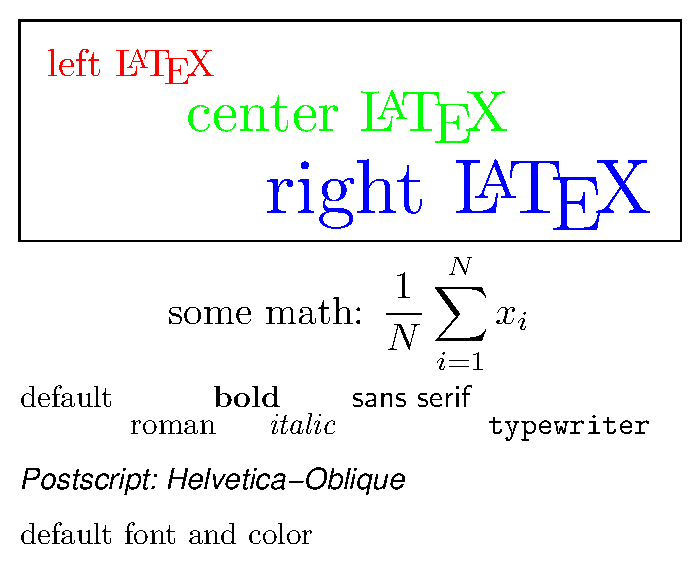
\includegraphics[width=0.5\textwidth]{figuras/test.eps}
	\caption[Curvas de transmissão dos filtros do \galex.]
	{Curvas de transmissão dos filtros do \galex, medidas em
	laboratório \citep{Morrissey2005}.}
	\label{fig:GalexFilters}
\end{figure}



Os {\em surveys} do \galex foram planejados de forma a se valer de outros {\em
surveys} já existentes em outros comprimentos de onda. A figura
\ref{fig:GalexSDSSOverlap} mostra a sobreposição dos {\em
footprints}\footnote{TODO: Foot.} dos surveys AIS e MIS do \galex e do {\em
Sloan Digital Sky Survey} (SDSS). Os objetivos primários da missão do \galex são
a calibração da taxa de formação estelar no universo local, e então determinar o
histórico cosmológico de formação estelar entre os redshifts $0 < z < 2$
\citep{Martin2005}. A comparação com dados de surveys em outros comprimentos de
onda tem um papel fundamental no cumprimento deste objetivo.

% FIXME: Adicionar figura.
\begin{figure}
	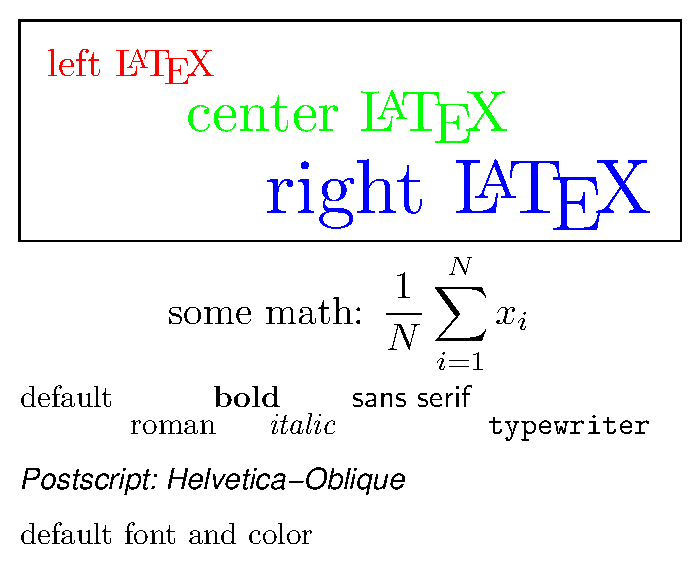
\includegraphics[width=0.5\textwidth]{figuras/test.eps}
	\caption[Footprint dos surveys \galex AIS, MIS e SDSS]
	{Footprint dos surveys \galex AIS, MIS (GR2+3) e SDSS (DR6),
	conforme \cite{Budavari2009}}
	\label{fig:GalexSDSSOverlap}
\end{figure}



%***************************************************************%
%                                                               %
%                Galex - O céu no ultravioleta                  %
%                                                               %
%***************************************************************%

\section{O céu no ultravioleta}
\label{sec:Galex:CeuUV}

% TODO: Escrever sobre céu no UV.
Copiar e colar 1.2 do \cite{Martin2005}.


%***************************************************************%
%                                                               %
%                     Galex - Resultados obtidos                %
%                                                               %
%***************************************************************%

\section{Resultados obtidos}
\label{sec:Galex:Resultados}

Galex papers. \cite{Wyder2007} + II e III. Adicionar um diagrama cor-mag. Falar
da bimodalidade. Conclusões dos principais artigos.

%***************************************************************%
%                                                               %
%                     Galex - Banco de dados                    %
%                                                               %
%***************************************************************%

\section{Banco de dados}
\label{sec:Galex:BancoDeDados}

Data releases. Legado. Referências com links em footnotes.

% End of this chapter
